\section{Elementos de la instalación}\label{sec:instalacion}

\subsection{Estructura de montaje}

Los cuatro módulos se colocan en una fila, en vertical, sobre la cara este del techo y paralelos a la lámina, con la misma inclinación de \SI{12}{\degree}. Se usan dos rieles de aluminio Unirac SM, uno por cada mitad del módulo, sujetos a las clavadoras del techo con soportes tipo L atornillados a través de la lámina ondulada, con arandela y sello en cada perforación. Los módulos se fijan a los rieles con grapas intermedias, que además unen eléctricamente el marco al riel para la puesta a tierra, y con grapas de extremo. La Tabla~\ref{tab:montaje} presenta la lista de materiales.

\begin{table}[!htb]
\caption{Materiales de la estructura de montaje (una fila de 4 módulos)}
\label{tab:montaje}
\centering
\footnotesize
\setlength{\tabcolsep}{3pt}
\begin{tabular}{l l r}
\toprule
Elemento & Referencia & Cant. \\
\midrule
Riel de aluminio de \SI{6.1}{m}, cortado a \SI{4.7}{m} & Unirac \textit{SM Rail} 240" & 2 \\
Grapa intermedia con unión a tierra & Unirac \textit{SM BND Midclamp} & 6 \\
Grapa de extremo & Unirac \textit{SM Endclamp} & 4 \\
Soporte tipo L, con tornillo y sello a la clavadora & Unirac \textit{L-Foot} & 10 \\
Terminal de tierra para riel & \textit{Lay-in lug} & 2 \\
\bottomrule
\end{tabular}
\end{table}

La cantidad de soportes se estimó con uno cada \SI{1.2}{m} de riel, cinco por riel. La separación final depende de la distancia entre las clavadoras del techo, que debe medirse en el sitio. Los módulos y la estructura agregan unos \SI{90}{kg} sobre \SI{8}{m^2} de techo, unos \SI{11}{kg/m^2}; falta verificar con el grupo el estado de las clavadoras y de la lámina antes de la instalación.

\subsection{Cableado}

Las longitudes de los tramos son supuestas, porque aún no se ha definido la ruta: \SI{10}{m} desde los módulos hasta los equipos, \SI{1.5}{m} entre la caja combinadora, el regulador y la barra DC, \SI{1}{m} entre cada batería y la barra, \SI{2}{m} entre la barra y el inversor, y \SI{5}{m} entre el inversor y los tableros. La corriente de diseño se calculó como $i_w=1.25\cdot1.25\cdot I_{sc}$ en los circuitos fotovoltaicos y como $i_w=1.25\cdot I_{\max}$ en los demás. Para el inversor, $I_{\max}$ es la corriente DC a su potencia continua, $2400/(0.94\cdot22.4)=\SI{114}{A}$, con \SI{22.4}{V} como tensión del banco casi descargado (\SI{2.8}{V} por celda, supuesto) \cite{nec2014}. La capacidad de los conductores se tomó de la Tabla 310.15(B)(16) del NEC 2014, la edición oficializada en Costa Rica \cite{codigo_electrico, nec2014}, y la caída de tensión se calculó con
\begin{equation}
\Delta V = 2\,L\,I\,R,
\end{equation}
donde $L$ es la longitud del tramo, $I$ la corriente y $R$ la resistencia del conductor por unidad de longitud (NEC, Cap.~9, Tabla 8). La Tabla~\ref{tab:cables} presenta el resultado.

\begin{table}[!htb]
\caption{Conductores por tramo}
\label{tab:cables}
\centering
\footnotesize
\setlength{\tabcolsep}{2.5pt}
\begin{tabular}{c l c c c c c}
\toprule
Tramo & Recorrido & $L$ [m] & $i_w$ [A] & Conductor & Capacidad [A] & $\Delta V$ [\%] \\
\midrule
T1 & Cadena -- caja combinadora & 10 & 22.5 & 10 AWG PV Wire & 26.2 & 1.82 \\
T2 & Caja combinadora -- regulador & 1.5 & 45.0 & 8 AWG THHN & 50 & 0.35 \\
T3 & Regulador -- barra DC & 1.5 & 106.2 & 2 AWG & 115 & 0.67 \\
T4 & Batería -- barra DC (cada una) & 1 & 96.9 & 2 AWG & 115 & 0.41 \\
T5 & Barra DC -- inversor & 2 & 142.5 & 2/0 AWG & 175 & 0.60 \\
T6 & Tablero principal -- inversor & 5 & 31.2 & 8 AWG THHN & 50 & 0.52 \\
T7 & Inversor -- subtablero crítico & 5 & 31.2 & 8 AWG THHN & 50 & 0.52 \\
\bottomrule
\end{tabular}
\\[2pt]
{\footnotesize $\Delta V$: T1 y T2 con $I_{mp}$ y $V_{mp}$ a \SI{63.2}{\celsius}; T3 con \SI{85}{A}; T4 con el doble de la parte de una batería; T5 con \SI{114}{A}; T6 y T7 con \SI{25}{A} a \SI{120}{V}.}
\end{table}

En el tramo T1 la corriente de diseño es $1.25\cdot1.25\cdot\SI{14.39}{A}=\SI{22.5}{A}$, con la $I_{sc}$ a \SI{63.2}{\celsius}. Se usa \textit{PV Wire} de 10 AWG, que admite \SI{40}{A} a \SI{90}{\celsius}; con las dos cadenas en una sola canalización (4 conductores, factor 0.80) y una temperatura sobre el techo de hasta \SI{50}{\celsius} (factor 0.82), su capacidad es de \SI{26.2}{A}. En T2 las dos cadenas ya están en paralelo y $i_w=\SI{45.0}{A}$. En T3 se usa la corriente máxima del regulador, \SI{85}{A}, y el calibre 2 AWG es el mayor que admiten sus terminales \cite{victron_mppt}. En T4, la corriente máxima del banco, \SI{155}{A}, es la carga simultánea del regulador y del cargador del inversor; cada batería lleva un cuarto, y por si el reparto no es parejo se dimensionó con el doble, \SI{77.5}{A}. Los cuatro cables T4 deben tener la misma longitud para que las baterías se repartan la corriente. En T5, $i_w=1.25\cdot\SI{114}{A}=\SI{142.5}{A}$, y el 2/0 AWG admite \SI{175}{A}. En la parte de corriente alterna, la corriente máxima del inversor es $\SI{3000}{VA}/\SI{120}{V}=\SI{25}{A}$.

La caída de tensión del lado fotovoltaico, sumando T1, T2 y T3, es de 2.84\,\%, y la del lado de alterna, de 0.52\,\% por tramo. Las dos quedan por debajo del 3\,\% por circuito que recomienda el NEC \cite{nec2014}. El tramo T1 es el de mayor caída; si la distancia real supera los \SI{10}{m}, conviene usar 8 AWG.

\subsection{Protecciones}

La Tabla~\ref{tab:protecciones} presenta las protecciones. Con solo dos cadenas no se requieren fusibles de cadena: si una cadena falla, la corriente inversa máxima que recibe es la de la otra, $1.25\cdot\SI{14.12}{A}=\SI{17.7}{A}$, menor que los \SI{25}{A} del fusible máximo en serie del módulo \cite{aiko_ds, nec2014}. En la entrada fotovoltaica del regulador se instala un protector de falla a tierra con interruptor, que sirve además como medio de desconexión del arreglo, y en la caja combinadora un descargador de sobretensiones de \SI{115}{V}, mayor que los \SI{84.6}{V} del arreglo en frío.

En el lado de las baterías, cada batería tiene su interruptor de \SI{100}{A}, que protege su conductor de 2 AWG (\SI{115}{A}) y permite desconectarla sin apagar el sistema. El interruptor de la salida del regulador es de \SI{125}{A}, el valor normalizado siguiente a la capacidad de \SI{115}{A} del conductor, como permite el NEC \cite{nec2014}, y el de la entrada del inversor es de \SI{175}{A}, igual a la capacidad del 2/0 AWG. La corriente del banco durante el arranque de los compresores, \SI{77.3}{A}, es menor que la de cualquiera de estos interruptores. En el lado de alterna, la entrada del inversor se alimenta desde un interruptor de \SI{40}{A} en el tablero principal, y el subtablero de cargas críticas tiene un interruptor principal de \SI{40}{A}; los circuitos existentes de refrigeración, iluminación y tomas se trasladan a ese subtablero con sus propios interruptores.

\begin{table}[!htb]
\caption{Lista de protecciones}
\label{tab:protecciones}
\centering
\footnotesize
\setlength{\tabcolsep}{3pt}
\begin{tabular}{l l c}
\toprule
Ubicación & Protección & Cant. \\
\midrule
Caja combinadora & Descargador DC MidNite MNSPD-115 & 1 \\
Entrada FV del regulador & Protector de falla a tierra MidNite MNDC-GFP80 (\SI{80}{A}, \SI{150}{V}) & 1 \\
Salida del regulador & Interruptor DC MidNite MNEDC125 (\SI{125}{A}) & 1 \\
Cada batería & Interruptor DC MidNite MNEDC100 (\SI{100}{A}, \SI{150}{V}) & 4 \\
Entrada DC del inversor & Interruptor DC MidNite MNEDC175 (\SI{175}{A}, \SI{125}{V}) & 1 \\
Inversor & Corte por baja tensión, sobrecarga y cortocircuito (integrados) & -- \\
Tablero principal & Interruptor 1P \SI{40}{A} Square D QO140 & 1 \\
Subtablero crítico & Interruptor principal 1P \SI{40}{A} Square D QO140 & 1 \\
Puesta a tierra & Marcos, rieles, gabinetes y polo negativo del banco, Cu 8 AWG & -- \\
\bottomrule
\end{tabular}
\end{table}

\subsection{Diagrama unifilar}

La Fig.~\ref{fig:unifilar} presenta el diagrama unifilar del sistema con la simbología de la norma IEC 60617.

\begin{sidewaysfigure}
\centering
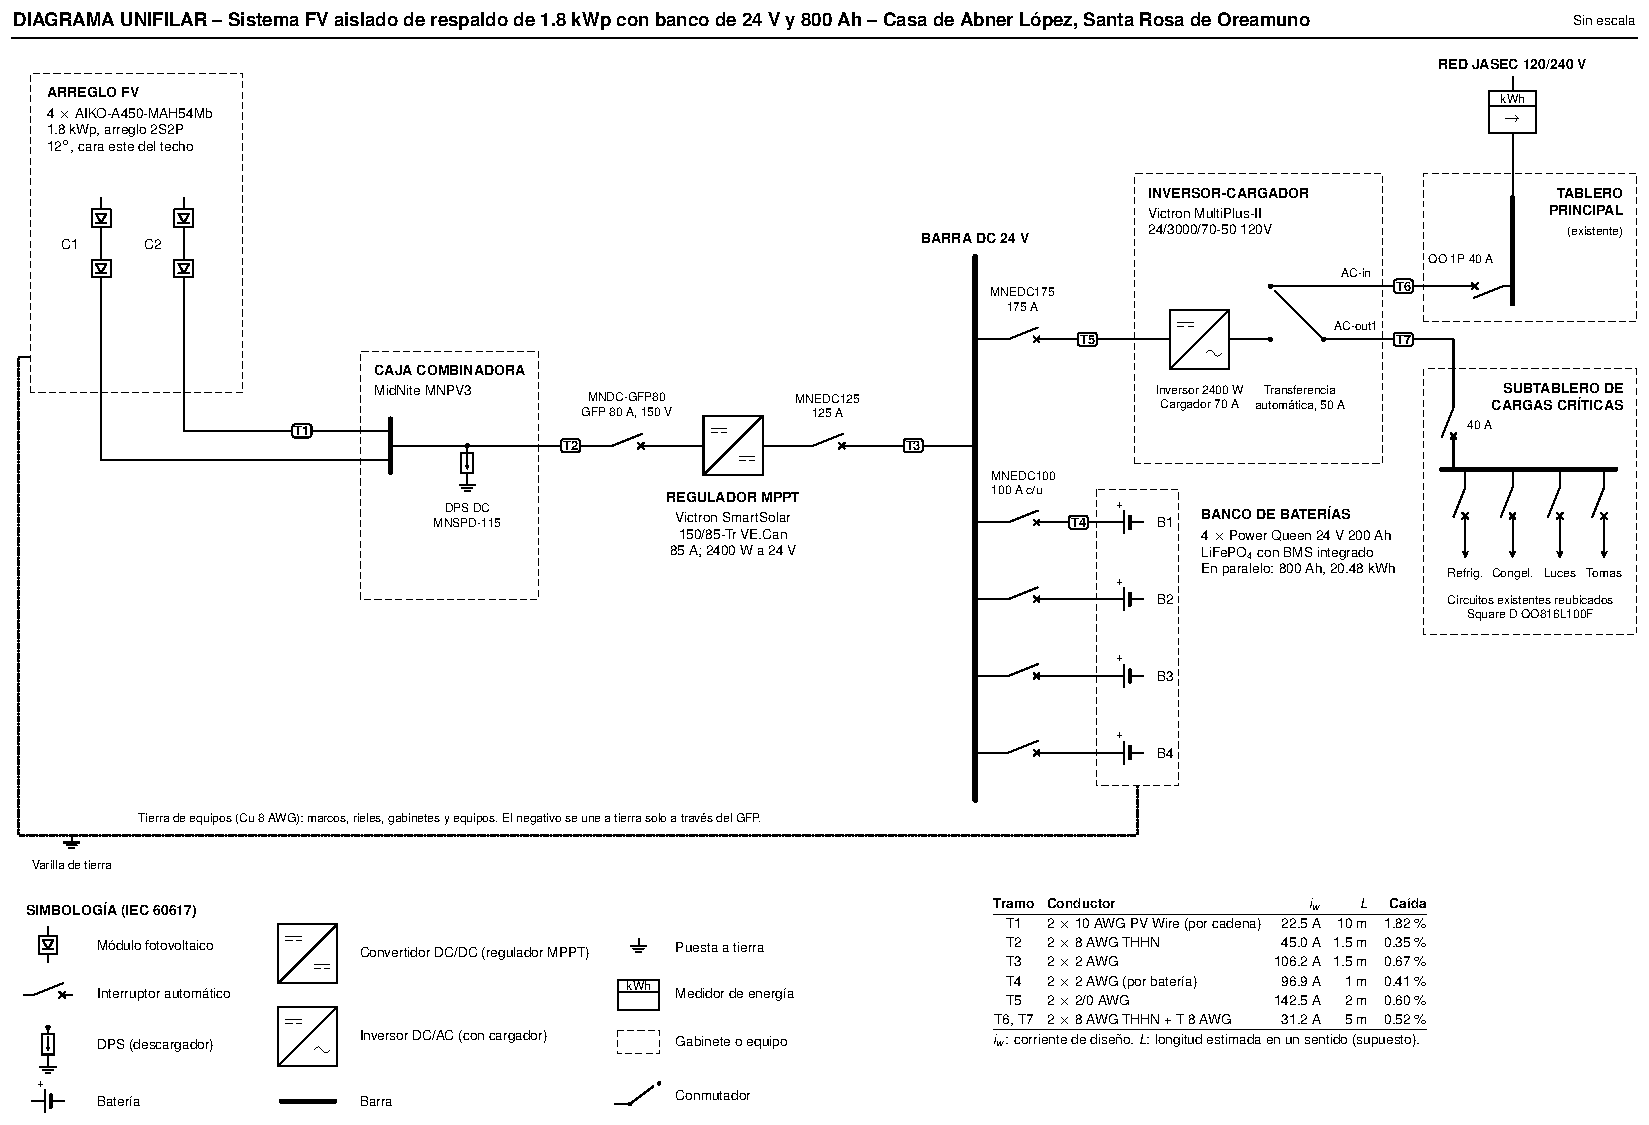
\includegraphics[width=\textheight]{unifilar_tikz.pdf}
\caption{Diagrama unifilar del sistema aislado de respaldo.}
\label{fig:unifilar}
\end{sidewaysfigure}
